% ---------------------------------------------------------------------------
% Author guideline and sample document for EG publication using LaTeX2e input
% D.Fellner, v1.13, Jul 31, 2008

\documentclass{egpubl}
\usepackage{eurovis2015}

% --- for  Annual CONFERENCE
% \ConferenceSubmission   % uncomment for Conference submission
% \ConferencePaper        % uncomment for (final) Conference Paper
% \STAR                   % uncomment for STAR contribution
% \Tutorial               % uncomment for Tutorial contribution
% \ShortPresentation      % uncomment for (final) Short Conference Presentation
% \Areas                  % uncomment for Areas contribution
% \MedicalPrize           % uncomment for Medical Prize contribution
% \Education              % uncomment for Education contribution
%
% --- for  CGF Journal
% \JournalSubmission    % uncomment for submission to Computer Graphics Forum
% \JournalPaper         % uncomment for final version of Journal Paper
%
% --- for  CGF Journal: special issue
% \SpecialIssueSubmission    % uncomment for submission to Computer Graphics Forum, special issue
\SpecialIssuePaper         % uncomment for final version of Journal Paper, special issue
%
% --- for  EG Workshop Proceedings
% \WsSubmission    % uncomment for submission to EG Workshop
% \WsPaper         % uncomment for final version of EG Workshop contribution
%
 \electronicVersion % can be used both for the printed and electronic version

% !! *please* don't change anything above
% !! unless you REALLY know what you are doing
% ------------------------------------------------------------------------

% for including postscript figures
% mind: package option 'draft' will replace PS figure by a filname within a frame
\ifpdf \usepackage[pdftex]{graphicx} \pdfcompresslevel=9
\else \usepackage[dvips]{graphicx} \fi

\PrintedOrElectronic

% prepare for electronic version of your document
\usepackage{t1enc,dfadobe}

\usepackage{egweblnk}
\usepackage{cite}

% For backwards compatibility to old LaTeX type font selection.
% Uncomment if your document adheres to LaTeX2e recommendations.
% \let\rm=\rmfamily    \let\sf=\sffamily    \let\tt=\ttfamily
% \let\it=\itshape     \let\sl=\slshape     \let\sc=\scshape
% \let\bf=\bfseries

% end of prologue

%\input{EGauthorGuidelines-body.inc}

\title[Visualization systems in Urban Planning related tasks]%
      {Visualization systems in Urban Planning related tasks}

% For anonymous conference submission, please enter your SUBMISSION ID.
\author[Shi Yin]
       {Shi Yin
       \\Electronic Visualization Laboratory
       \\Department of Computer Science
       \\University of Illinois at Chicago}

%% For the final version of your accepted paper, please enter the authors names and affiliations.
%\author[D. Fellner \& S. Behnke]
%       {D.\,W. Fellner\thanks{Chairman Eurographics Publications Board}$^{1,2}$
%        and S. Behnke$^{2}$
%        \\
%         $^1$TU Darmstadt \& Fraunhofer IGD, Germany\\
%         $^2$Institut f{\"u}r ComputerGraphik \& Wissensvisualisierung, TU Graz, Austria
%       }

% ------------------------------------------------------------------------

% if the Editors-in-Chief have given you the data, you may uncomment
% the following five lines and insert it here
%
% \volume{27}   % the volume in which the issue will be published;
% \issue{1}     % the issue number of the publication
% \pStartPage{1}      % set starting page


%-------------------------------------------------------------------------
\begin{document}

% \teaser{
%  
\includegraphics[width=\linewidth]{eg_new}
%  \centering
%   \caption{New EG Logo}
% \label{fig:teaser}
% }

\maketitle

\begin{abstract}
In this report, we survey a variety of visulaization systems in different domains related to urban planning, including Geographical Information Systems, Urban Search \& Rescue systems, and urban simulation systems.
\end{abstract}

%-------------------------------------------------------------------------
\section{Introduction}
Urban planning is a technical and political process concerned with the use of land and design of the urban environment, including economy, environment, transportation and distribution networks, etc.

The modern origins of urban planning lie in the movement for urban reform that arose as a reaction against the disorder of the industrial city in the mid-19th century. Urban planning can include urban renewal, by adapting urban planning methods to existing cities suffering from decline. Alternatively, it can concern the massive challenges associated with urban growth, particularly in the Global South.[2]

Visualization has always been of significant importance in geographic related fields ~\cite{al1999using}. Good visualization makes analyzing and investigating collected geospatial data simpler and more efficiently thus enabling a deeper and more organized understanding and more effective application into practice.

In this report, we survey the state-of-the-art in visualization systems in a variety of urban planning related fields. In Section 2, we discuss Geographical Information Systems and online Mapping APIs. In Section 3, we introduce an application of visualization in Urban Search \& Rescue Mission planning. In Section 4, we take a look at an urban visualization system built upon urban simulation software. In Section 5, we include two interviews of domain scientists. In Section 6, we conclude the report.

%-------------------------------------------------------------------------
%\section{Urban Accessibility}

%-------------------------------------------------------------------------
\section{Geographic Information Systems Using Google Maps API}

Geographic Information Systems (GIS) is probably the most popular and the most famous visualization system that are used by urban planning researchers, professionals and students to process, manipulate, manage, and visualize geographical information data, and known by researchers from other research areas.

Online mapping APIs are new tools that emerged only in recent years. The advantages of them are: 1. \textbf{free for use}. Most APIs are provided to any user for free, while some are not, or have limited functionality in free version. For example, ArcGIS has a Javascript API, which is not as powerful as its desktop mapping software ArcGIS for Desktop and its mapping servicer software ArcGIS for Server, but includes most of the frequently used functionality. 2. \textbf{easy-to-use}. Most APIs are well documented and organized. 3. \textbf{scalability}. Some of online mapping APIs, such as Google Maps API, Bing Maps API, are providing limited version for free use, and provided also non-free versions for users with special needs.

Each API is actually with significant difference from each other in terms of weight (lightweight/heavyweight), scalability (small amount of data/large amount of data), functionality (simple-and-frequent-tasks-only/all-in-one) while at the same time keeps the similarity in that 1) the supported data is similar and 2) task sets are similar.

Here we list some interesting work that facilitates GIS and/or Google Maps API to visualize geographical urban data to give readers an understanding of the range of applications.

\subsection{logistics network system}
In ~\cite{fu2010logistics}, the authors introduced a logistics network system built upon Google Maps API. The major features of Google Maps API utilized by this system include: basics functions of mapping, including the map layers and UI controls; event-driven asynchronous HTTP communication that interact with Google Maps API, and geocoding service that allows converting address to coordinates.

The system consists of 5 modules. \textbf{Registration module} and \textbf{Information Publishing module} are for administrative purposes and we omit them here. \textbf{Transaction module} and \textbf{Information Query and Matching module} are to match the vehicle and cargo based on a series of parameters such as the vehicle's location, cargo types, cargo weight and route, and then saves the transaction information into the database, waiting for monitoring and other queries.

The last module, \textbf{Map Service module} is the major module of the system. This module itself includes 4 sub-modules. \textbf{Querying sub-module}, which provides functionality for the vehicle owner or the cargo owner to conduct historical information management, and \textbf{Navigating sub-module}, whose primary function is to supply the vehicle owners and the drivers with map navigation, are with no significant interest.

The more important sub-module of this system as a logistics management tool, is the \textbf{Monitoring sub-module} that is able to show real time location of vehicles and goods dynamically, as well as several previous checkpoints through the route. In the backend, this module receives GPS positioning data with real-time communication, processes it and stores it in the database awaiting for user's call.

\begin{figure}[htb]
  \centering
  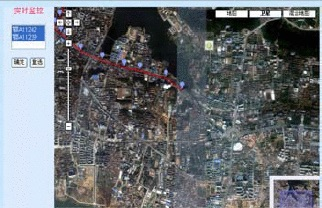
\includegraphics[width=.95\linewidth]{fig-3-1}
  \caption{\label{fig:fig-3-1} \textbf{Monitoring vehicles on Google Maps}}
\end{figure}

The fourth sub-module of Map Service module is \textbf{POI sub-module}, where Points of Interest associated with the logistics, such as large-scale logistics park, logistics companies, and distribution centers, are stored and ready to be displayed. Served as a auxiliary companion of \textbf{Monitoring sub-module}, POI sub-module enhances the usability of this system.

%-------------------------------------------------------------------------
\subsection{tourism information systems}
In ~\cite{wu2013design}, the author introduced their design and implementation of a tourism information system based on Google Maps API. The traditional way that a tourist collects tourism-related information, such as restaurants, hotels, attractions, transportation and entertainment, is by searching on different websites. Three deficiencies are within this traditional way of information collecting: 1) tourism information is scattered; 2) tourism information is unconfirmed; 3) tourism information is flat. This work is an attempt to solve these issues by building an integrated tourism information platform where tourists can conveniently obtain more references for their travel.

\begin{figure}[htb]
  \centering
  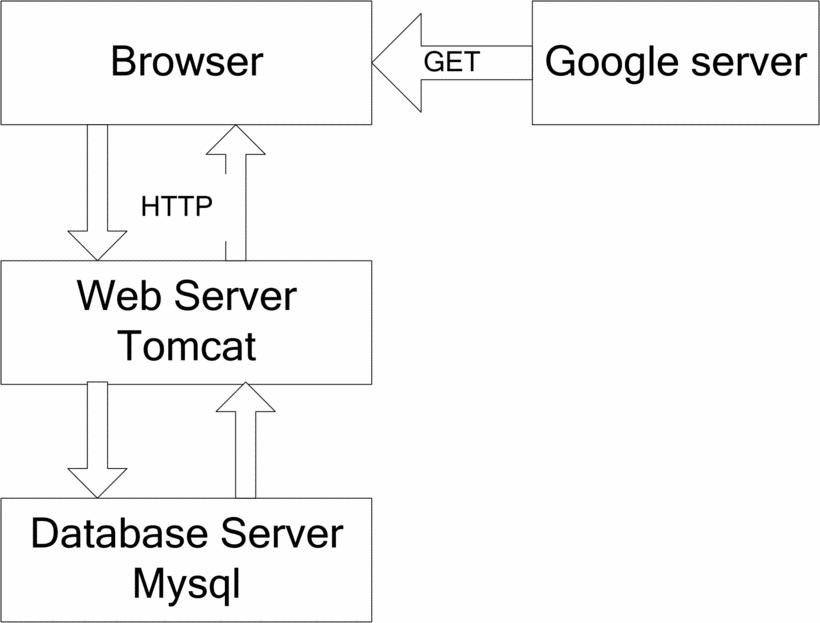
\includegraphics[width=.95\linewidth]{fig-3-2}
  \caption{\label{fig:fig-3-2} \textbf{Architecture diagram.}}
\end{figure}

A similar system for tourists is presented in ~\cite{pejic2009expert}. This system makes use of services made available through Google Maps API such as Geocoding which from given address returns a geolocation, Directions which provides routing instructions from a start point to a destination point, Streetview which shows virtual picture of locations, GoogleBar for local search of the map, and so on. The difference is that this platform not only provides basic mapping functionality but also integrated an expert system that can provide customized information to users.

%------------------------------------------------------------------------
\subsection{land use information release system}
In 2010, Zhang et al. ~\cite{zhang2010land} introduced a land use information release system. It uses Google Maps API for map service, XML for data storage. It has a three-layer architecture (data layer, business logic layer and presentation layer). It allows user to query land use information by selecting filters (text query), keyword search (local search), geocoding search (reverse address resolution). It also allows user to send feedback about each data feature on the map.

%------------------------------------------------------------------------
\subsection{railroad settlement information management system}
Also in 2010, Wang and Zhou ~\cite{wang2010settlement} proposed a railroad settlement information management system that makes use of similar techniques as ~\cite{zhang2010land}, such as Google Map Service, XML, Ajax, etc. The major difference is they provided a better front-end, which visulized data using traditional charts such as line charts and bar charts to perform analysis on the data.

\begin{figure}[htb]
  \centering
  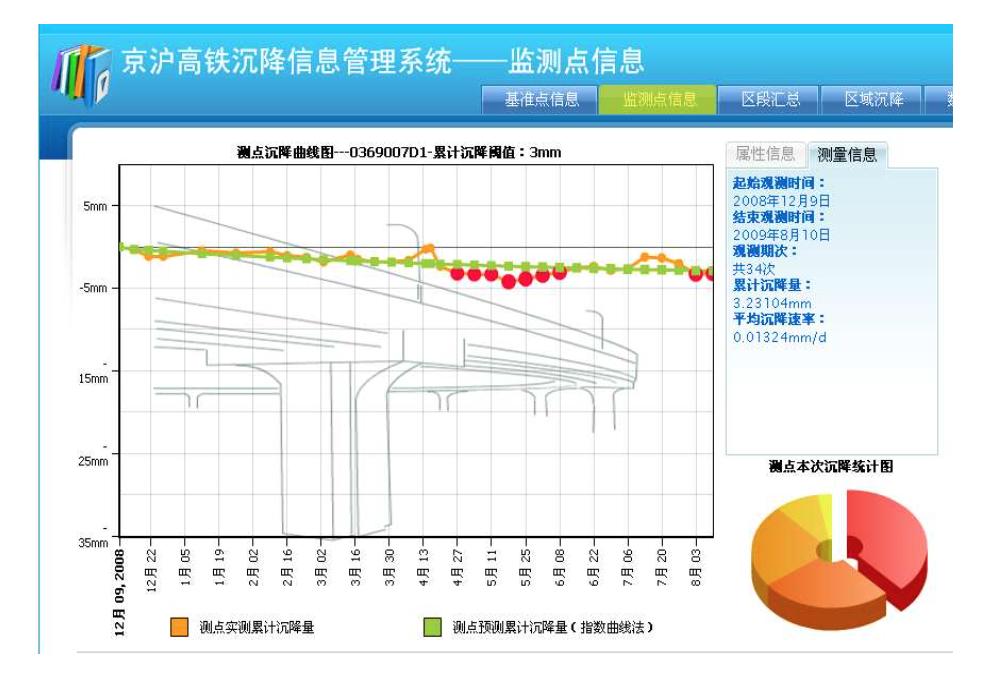
\includegraphics[width=.95\linewidth]{star-3-1}
  \caption{\label{fig:star-3-1} Search, warning and statistics of monitor point’s settlement information}
\end{figure}

\begin{figure}[htb]
  \centering
  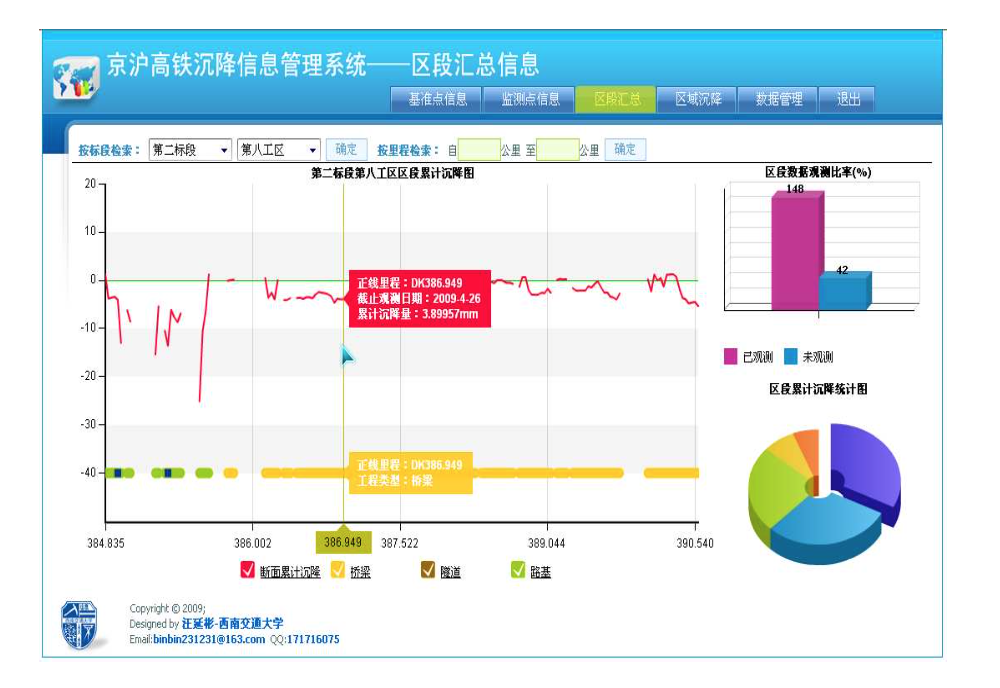
\includegraphics[width=.95\linewidth]{star-3-2}
  \caption{\label{fig:star-3-2} Statistical analysis of railway profile’s cumulative settlement information}
\end{figure}

%------------------------------------------------------------------------
\section{Urban Search \& Rescue Mission Planning system}
In an \textit{Urban Search \& Rescue} (USAR) operation, victims' survivability is mostly determined by the time-to-rescue. It is critical that medical attention or extraction be provided as fast as possible. As structural damage caused by disasters makes available floor plans outdated, it is very important that the \textit{Incident Commander} (IC) can analyze the available information and coordinate multiple rescue responders. In recent years, the traditional way of assessment where 2D maps of the collapsed buildings are hand-drawn based on the descriptions of rescue responders on site is replaced by unmanned robots equipped with sensors to detect victims, gather information about hazardous area, and perform scans of rooms to create a 3D point cloud of the building’s interior.

In 2014, Bock, A. et al. ~\cite{bock2014interactive} proposed a visualization system for IC to use in USAR scenarios. The system creates an interactive 3D rendering that increases the commander's spatial awareness of the building (Figure ~\ref{fig:star-4-1} (a-c) and Figure ~\ref{fig:star-4-3}) and supports the planning and analysis of available access paths that are automatically generated by the system based on varying risk factors (Figure ~\ref{fig:star-4-4}). Then IC uses this information to instruct rescue responders to reach \textit{Points of Interests} (POI). At the same time the IC is able to annotate the visualization with new information provided by the on-site responders and thus shift the decision making process from opportunistic to being strategical.

This is the first system facing post-disaster USAR scenarios that uses 3D point cloud for visualization. Before this system, most of visualization-oriented work published in the field is concerned with pre-disaster evacuation planning. Reddy et al. ~\cite{reddy2012visual} performed notable work based on analyzing possible bottlenecks of escape routes. Ribarsky et al. presented a system organizing first responders in intact structures ~\cite{ribarsky2010mobile}. Kim et al. developed a system enhancing the situational awareness of responders using a mobile visual analytics tool ~\cite{kim2008mobile}. As for post-disaster USAR planning, existing systems are mostly based on 2D representations ~\cite{kleiner2009operator}~\cite{pellenz2010stable}~\cite{wirth2007exploration}~\cite{dornhege2013frontier}.

\begin{figure*}[htb]
  \centering
  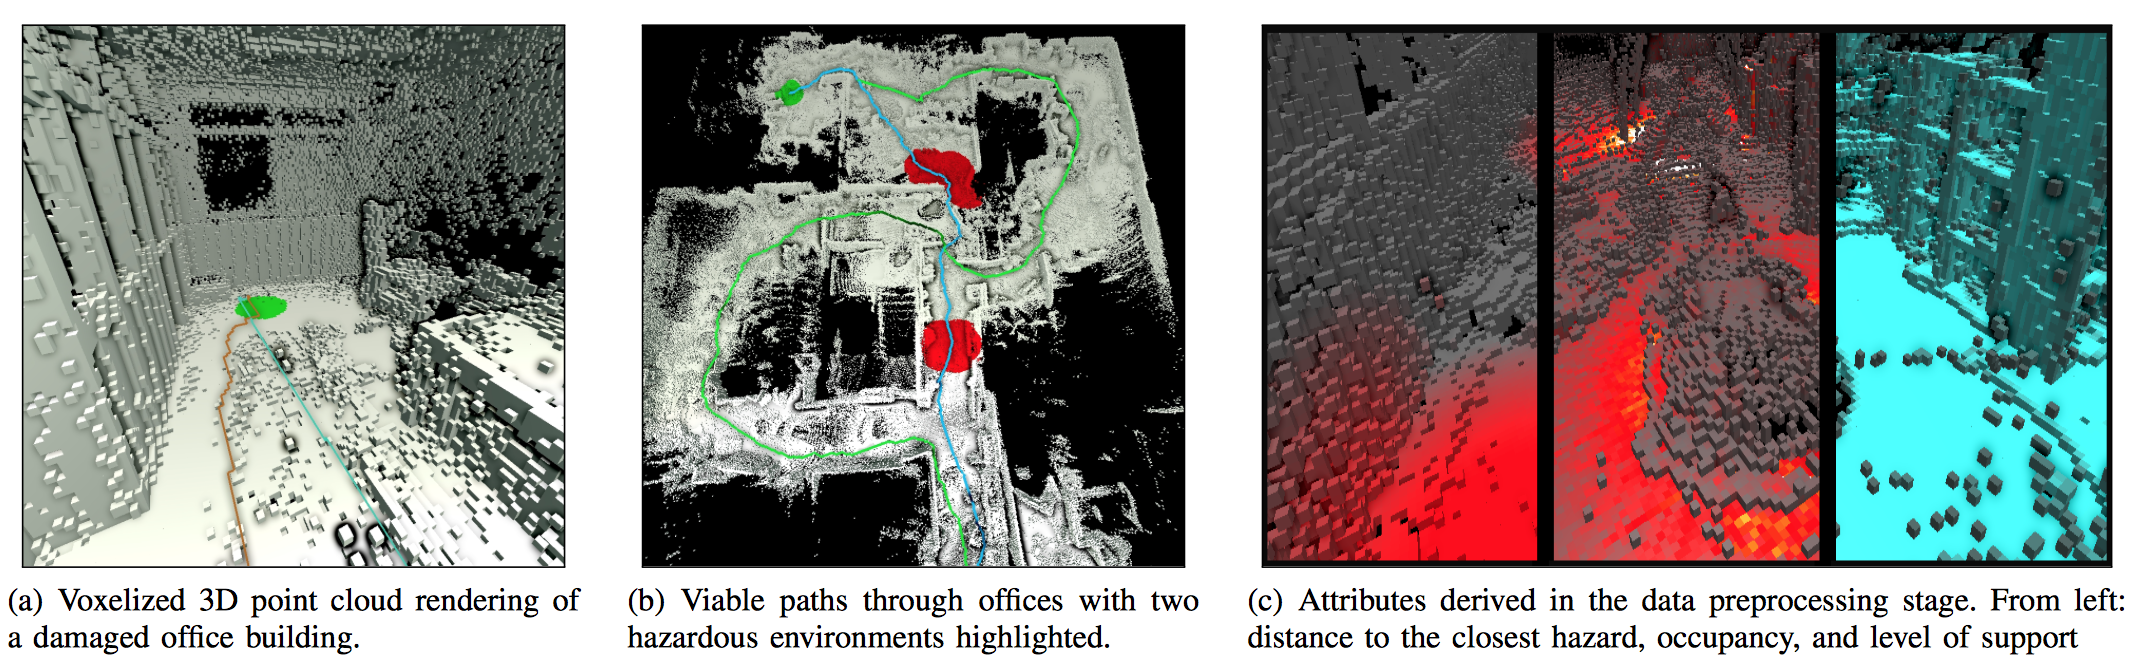
\includegraphics[width=.95\linewidth]{star-4-1}
  \caption{\label{fig:star-4-1} The system applied to a building at Tohoku University. Different views support a comprehensive understanding, allowing the IC to select and inspect paths that reach a Point of Interest, which are integrated into the rendering. Inspection and path computation is based on a set of derived attributes (c).}
\end{figure*}

\begin{figure}[htb]
  \centering
  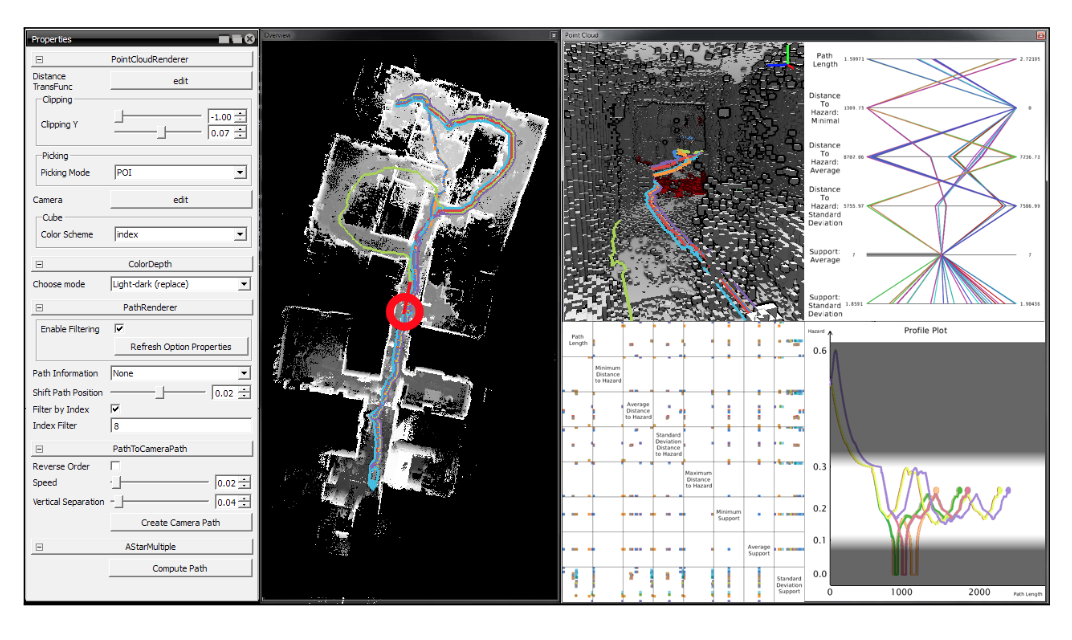
\includegraphics[width=.95\linewidth]{star-4-2}
  \caption{\label{fig:star-4-2} A screenshot showing the system for a typical scenario. each view can be maximized to fill the entire screen for in-depth inspection. An overview (left) shows a top-down view of the building to provide context, a multi-view (right) shows the different components of our system.}
\end{figure}

\begin{figure*}[htb]
  \centering
  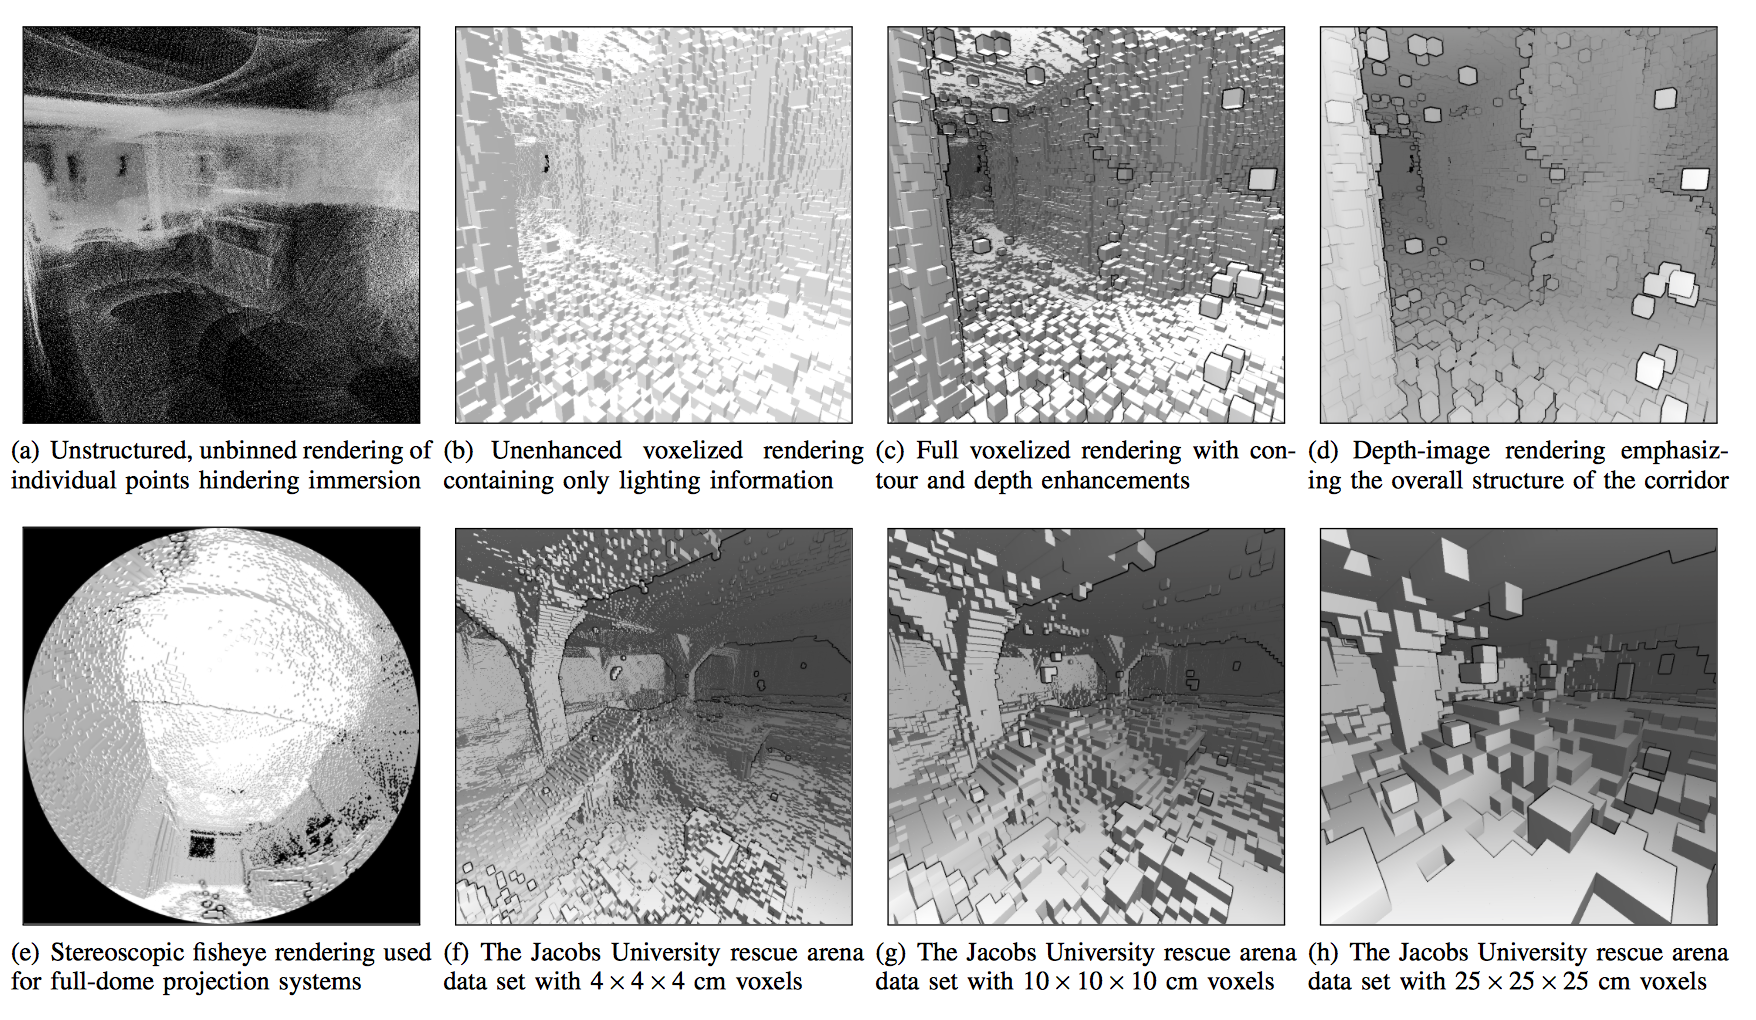
\includegraphics[width=.95\linewidth]{star-4-3}
  \caption{\label{fig:star-4-3} These images show different rendering techniques of the same location in the Tohoku dataset (a-d). Rendering the individual voxels as points does not allow for an immersive rendering as depth-cues are missing (a). Binning the point cloud and representing each voxel as a axis-aligned box solves this problem (b). In order to enhance the contours of the scene and produce a better immersion, image-space enhancements were performed (c). Alternatively, the IC can choose a rendering method imitating the output of range imaging cameras (d). It is possible to render the point cloud in stereoscopic fisheye that can be used for dome surfaces or VR glasses (e). The voxel size's effect during binning is shown for the rescue arena dataset (f-h).}
\end{figure*}

\begin{figure}[htb]
  \centering
  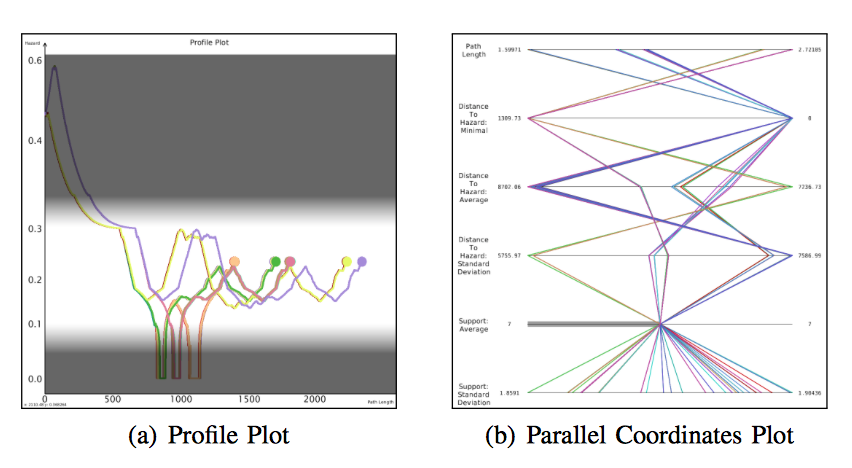
\includegraphics[width=0.95\linewidth]{star-4-4}
  \caption{\label{fig:star-4-4} \textbf{Views supporting comparative path analysis.} (a) the profile plot presents the change of an attribute along paths; here the distance to the closest hazard. (b) parallel coordinates plot showing correlations between attributes.}
\end{figure}


%------------------------------------------------------------------------
\subsection{side note about point cloud}
It is worth mentioning that there are not many applications we found in urban planning context that utilizes point cloud for 3D rendering. There are great potential in point cloud visualization in urban planning related tasks though, as large amount of fundamental research has been conducted, making point cloud ready-to-use.

There has been work by Richter et al. using a level-of-detail structure to render massive point clouds at high frame rates ~\cite{richter2010out}. Xu et al. showed that non-photorealistic rendering techniques can be applied to point cloud data ~\cite{xu2004stylized}. It is the contour lines in their rendering that inspired xx's rendering algorithm.
More recently, Pintus et al. presented a rendering algorithm that enhances features of unstructured point clouds in real-time without preprocessing ~\cite{Pintus:2011:RRM:2384495.2384513}. Some other work in this area that converts point cloud to surfaces, which is essential for urban modeling, include ~\cite{fabio2003point}, ~\cite{holzer2012adaptive} and ~\cite{nagai2015tomographic}. Last but not least, the widely used Point Cloud Library (PCL) ~\cite{rusu20113d} is also making major contribution to the increasing popularity of point cloud.

%------------------------------------------------------------------------
\section{Urban Modeling and Urban Simulation}
Another field in urban planning context where visualizing data plays a central role in research activity is urban simulation. The term **urban simulation** has two definitions in urban planning context. One common use of this term by domain scientists in urban planning is to describe 3D rendering of urban landscapes, like in ~\cite{fruh2003constructing}~\cite{merrell2007example}~\cite{muller2006procedural}~\cite{muller2007image}~\cite{parish2001procedural}~\cite{ribarsky2002urban}. Here in our discussion, we focus on the second definition though, where urban simulation is a behavioral or process modeling of the dynamic changes in urban activities and landscapes.

Urban simulation models and the visualization of their results have been increasingly used by planning agencies in city, county, and regional scopes to assess alternative transportation investments, land use regulations, and environmental protection policies.

There are two major challenges in urban simulation. The first and fundamental one is to adequately model and predict the complex socio-economic interactions that determine the growth of an urban space in order to simulate the change of this urban space over time. The future structure of a city is governed by both deterministic rules (e.g. population capacity of the city must grow) and organic rules (e.g. social, cultural, and economic interactions strongly influence how a city grows). Because of the intricate nature in urban simulation, a simulation model will usually generate an overwhelming amount of data when running over a long period of forecasting time in a large geographical scale (e.g., one or more decades for a large city with a several million population). This makes it difficult for researchers, planners, or policy-makers to interpret the data.

This is where the second challenge in urban simulation lies. An effective and intuitive visualization is essential to extract useful information from the large mass of data generated by such simulations. In fact, visualization has played an integral part in the development and use of urban simulations of different types for a while. Batty introduced various approaches that relate urban modeling, GIS, and computer graphics in ~\cite{batty1993urban} and described the impact of virtual reality and 3D visualization to GIS and demonstrated it in a variety of examples ~\cite{batty1997virtual}. Cartograms, which use map shape warping to visualize relationships and values of urban and geospatial datasets, is widely used ~\cite{dorling2006worldmapper}~\cite{hertzmann2001image}~\cite{panse2006visualization}~\cite{pinnel2000design}. Dykes and Brunsdon ~\cite{dykes2007geographically} introduced geowigs, a series of geographically weighted interactive graphics, to provide large-scale geographical environment visualization. Visualization has also been used for the purposes of education, exploration, explanation, and engagement ~\cite{batty2006visualization}. Some approaches also make use of choroplethic maps, generated by exporting simulation results to GIS for rendering.

Recently, Vanegas et al. ~\cite{vanegas2009visualization} introduced a method that automatically and interactively infers geometry and image content of urban layouts using the input data and output data of an urban simulation, pushing urban simulation and urban visualization one more step forward. The major contributions of their work are:
\begin{enumerate}
  \item A methodology for enhancing the visualization of the result of urban simulations by using inferred higher-level structural information.
  \item A set of automatic and interactive algorithms for generating a visually plausible urban layout from the data generated by an urban simulation.
\end{enumerate}

The input of this method consists of three components: the first one is a set of parcel and street geometries obtained from shapefiles from ArcGIS; the second is the high-resolution geo-referenced aerial imagery of the targeted area, in this case GeoTIFF files containing coordinates information; and the last is the socio-economic data of this area, which is used as input to an urban simulation engine, this case UrbanSim, that predicts the future value of several state variables of the urban space. These intermediate results of the simulation will then be used by the visualization tool to generate detailed urban layouts for any point in the simulation. The overall process of the pipeline is illustrated in Figure ~\ref{fig:star-5-1}.

\begin{figure*}[htb]
  \centering
  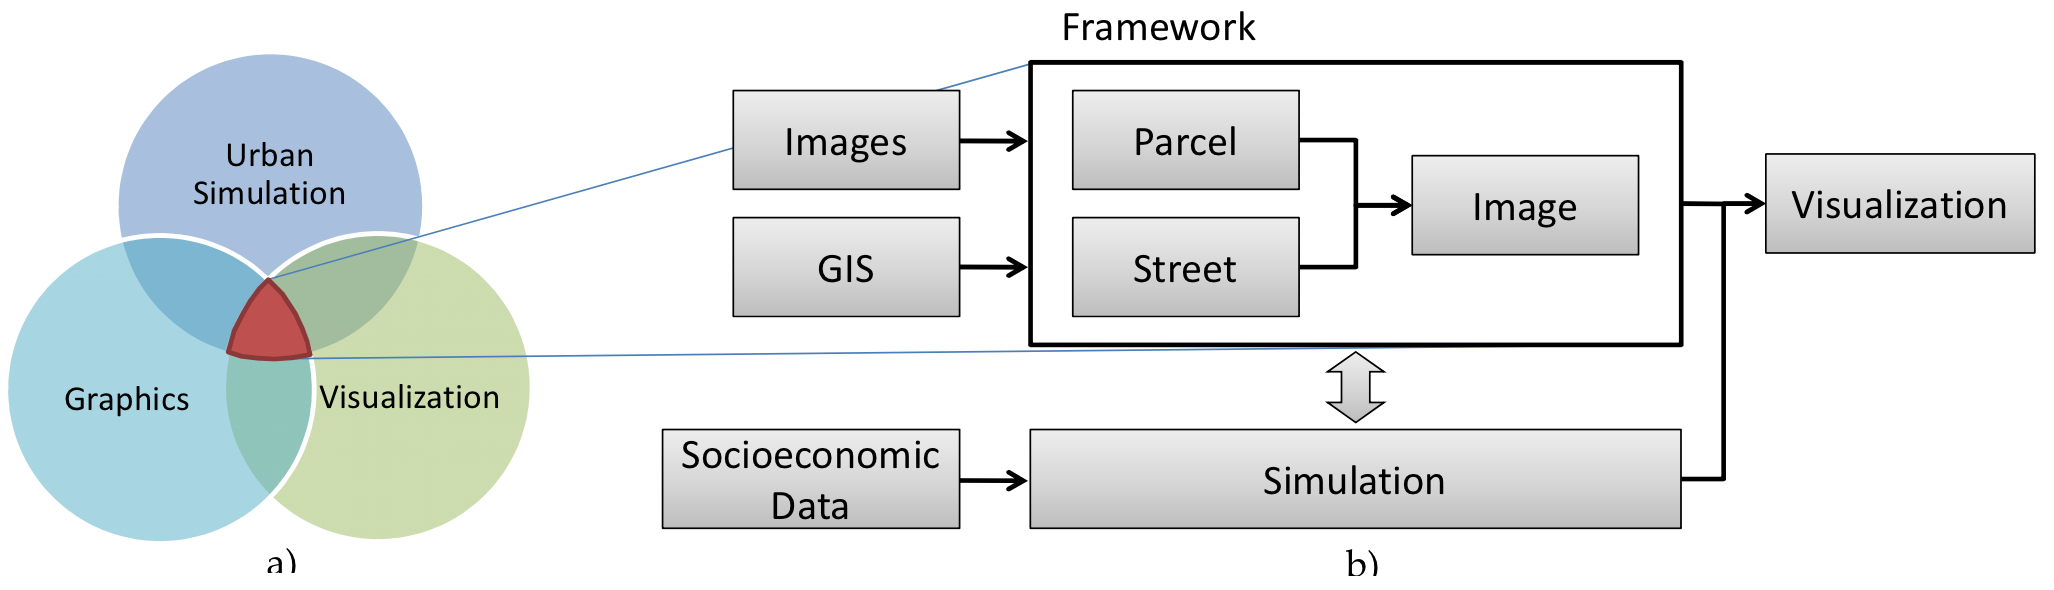
\includegraphics[width=.95\linewidth]{star-5-1}
  \caption{\label{fig:star-5-1} (a) This method is built upon the combination of urban simulation, urban visualization and computer graphics. (b) the processing pipeline completes an urban simulation with visualization. Images and GIS data, together with simulation results data, are fed into the framework to generate parcels and streets, which are then be used as basis for generating urban layout images.}
\end{figure*}

\subsection{simulation of urban spaces}

\subsection{layout generation}
Spatial transformations of parcels and of the buildings that occupy them can be inferred from the state variables of the urban simulation system. The transformations that frequently take place in the layout include the replacement of buildings with newer and/or larger structures, the division of a parcel into smaller parcels, and the creation of new streets. The visualization system can detect changes in user-defined state variables and translates such changes into transformations to the initial street and parcel information, and also to the fragments of aerial imagery associated to each transformed parcel.

This part is where the core visualization algorithm of the system lies. It can be divided into three steps: parcel generation, street generation and parcel-content generation.

\subsubsection{parcel generation}
The first step is to generate new parcels based on simulation results. How a parcel is partitioned is built upon some desired properties: (i) parcels generally have egress, (ii) city blocks are usually formed by rows of one or two parcels, and (iii) the contour of a parcel is most often a quadrilateral and often nearly rectangular.

Based on these properties, the system uses an recursive algorithm to partition an existing city block or a large parcel. Firstly, parcels whose population has changed (based on simulation data) are marked as candidate for subdivision. Then subdivision attempts start from the largest candidate parcel. A block-sized parcel is split into two parcels, each of which is recursively subdivided until reaching either the number of households specified by the simulation or a minimum parcel area, which is computed automatically as the mean parcel area of all parcels within a chosen distance threshold. If egress is desired (first property), a split is not made if resulting parcels will have no access to streets. This also makes sure that up to two rows of parcels are generated (second property). Since this algorithm works recursively, after a few subdivisions, most new parcels will be nearly rectangular (third property), even if the initial parcel is with complex contour.

\begin{figure}[htb]
  \centering
  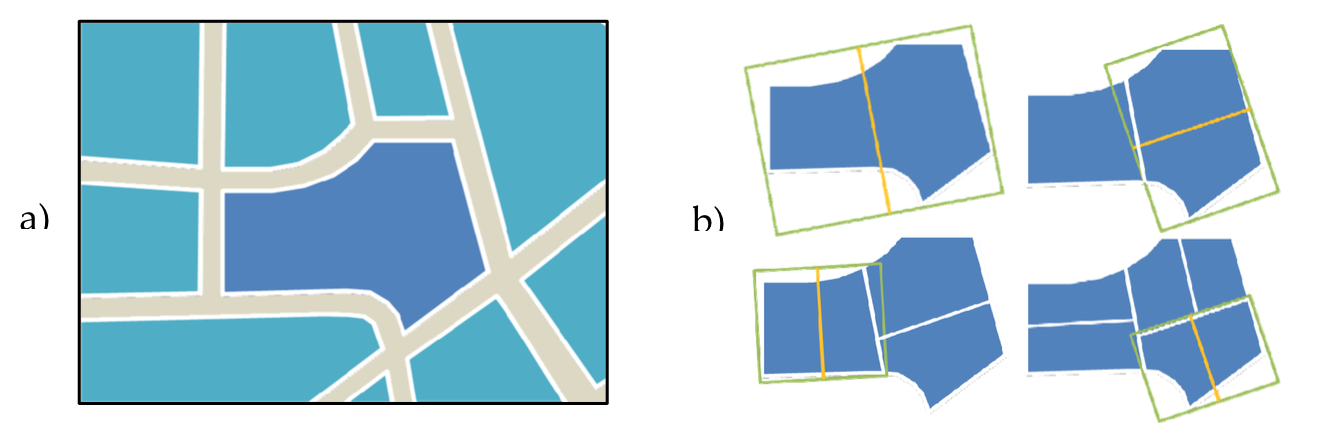
\includegraphics[width=.95\linewidth]{star-5-2}
  \caption{\label{fig:star-5-2} (a) A candidate large parcel corresponding to a city-block is divided into smaller parcels (beige=street, light blue=parcels/city-blocks, dark-blue=parcel to subdivide). (b) First four subdivisions of the original parcel yield to parcels with egress (green=oriented bounding box)}
\end{figure}

\subsubsection{street generation}
The second step is to generate streets. Parcel subdivision generates a subdivision line in each step. For street generation, decisions about whether the subdivision line corresponds to a new street segment or a new parcel boundary segment are made. To make the decision, the system takes the number of parcels per city-block, a value whether from simulation or specified by user, into consideration. When the subdivision line is selected to be a street segment, the system will make sure newly-generated city blocks has similar aspect ratio to that of nearby city blocks.

The geometry of a new street is obtained by perturbing the initial subdivision line segment, which is in fact a poly-line with a certain number of inner control points. These control points are used to make sure the new street segment is similar to the streets in nearby area. In this step, each initial large parcel is subdivided independently, and further processing is conducted to prevent too many deadends or T-intersections. When endpoints of two street segments are close and the turning angle is not too sharp, they are joined to form a single longer street segment.

This step uses the same stop condition as the first step. The result of this process is a new network of parcels and streets that can be output in vector format. Figure 5.3 shows an example of the recursive process, where the target number of additional parcels is twelve and the chosen approximate number of parcels per city block is four.

\begin{figure}[htb]
  \centering
  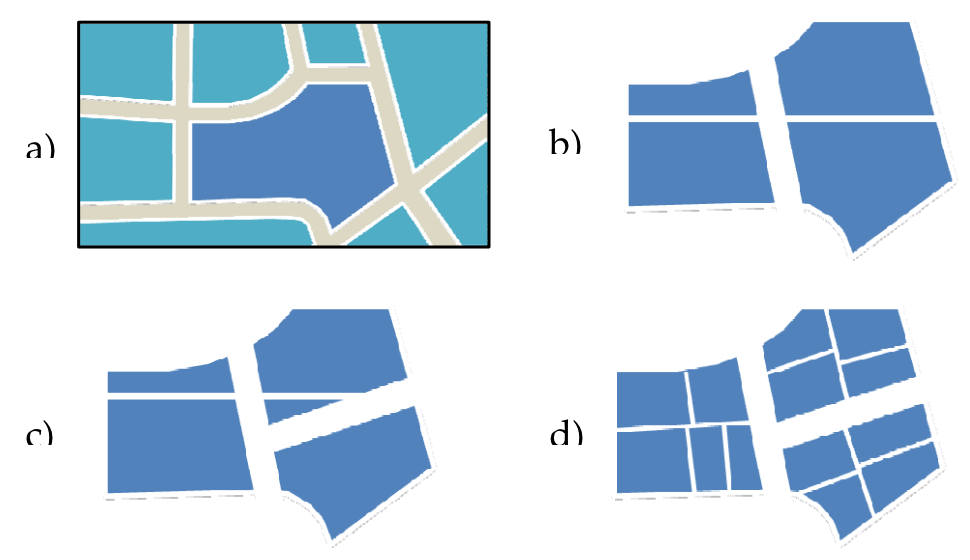
\includegraphics[width=.95\linewidth]{star-5-3}
  \caption{\label{fig:star-5-3} (a) An initial parcel (from Figure 4). (b-c) First two subdivisions are chosen to be streets. (d) In further iterations, only more parcels per city-block are produced.}
\end{figure}

\subsubsection{parcel-content generation}
The last step of layout generation is to generate plausible image content for each of the newly generated parcels. The way to do this is to reuse existing aerial image fragments of parcels with similar characteristics. The similarity metric is defined as the weighted sum of the similarity of the simulation state values (e.g. households per parcel, year of the construction for buildings, zoning classification, etc) and similarity of geometric shape (e.g. area, aspect ratio, etc).

Since the number of vertices of the source and destination parcels does not necessarily match, a image-wraping algorithm is used to warp an \textit{a}-sided polygon to \textit{b}-sided polygon. The selected source image fragment is texture-mapped onto the destination parcel geometry and rendered together with the rest of the layout. Oriented-bouding box of both source parcel and destination parcel are partitioned into scan lines perpendicular to their longest axis. A fixed number of points is regularly spaced and the points are generated along both scan lines and culled to be inside each respective polygon. These points correspond one-to-one. The process is repeated for each scan line. The destination parcel is rendered using (i) the coordinates of the points to define a quadrilateral mesh and (ii) the coordinates of the corresponding source parcel quadrilateral mesh to make texture coordinates.

\begin{figure}[htb]
  \centering
  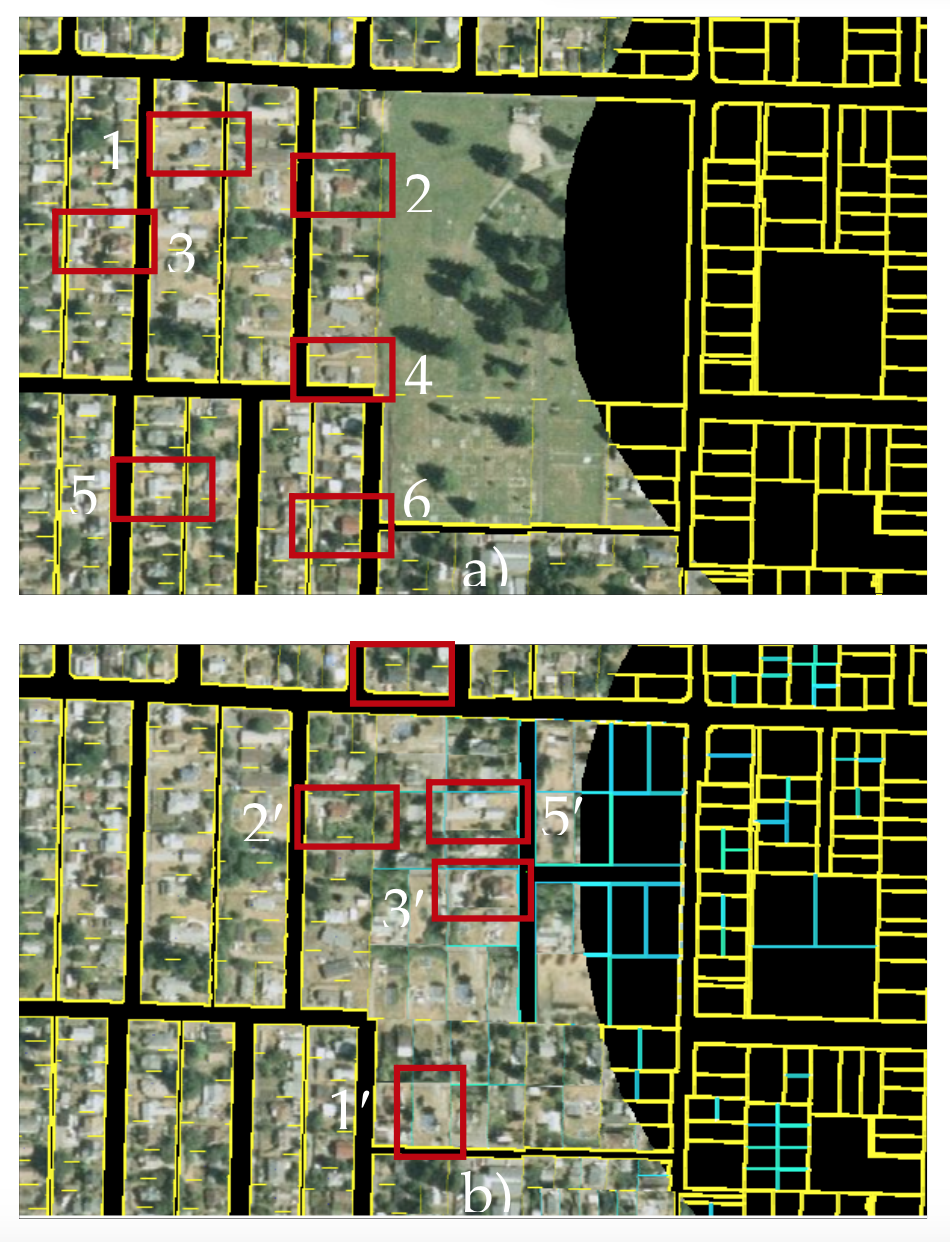
\includegraphics[width=.95\linewidth]{star-5-4}
  \caption{\label{fig:star-5-4} (a) An original urban area from where parcel image fragments are extracted; (b) The newly generated area, with some of reused image content highlighted.}
\end{figure}

\subsection{rendering and user interaction}
The system enables the visualization of the simulation results using a variety of rendering methods, such as rainbow maps and choroplethic maps, to display one of several simulation variables, such as house holds, buildings, distance to large streets, distance to highways, land value, and year built of the constructions, etc. (See Figure ~\ref{fig:star-5-6})

The system loads the data within the current field-of-view dynamically, allowing user to explore the dataset freely. The whole process is fully automatic, with only minimal selection of the simulation variables and visualization methods. This simplifies the visualization task and makes a web-based viewing program possible.

\begin{figure*}[htb]
  \centering
  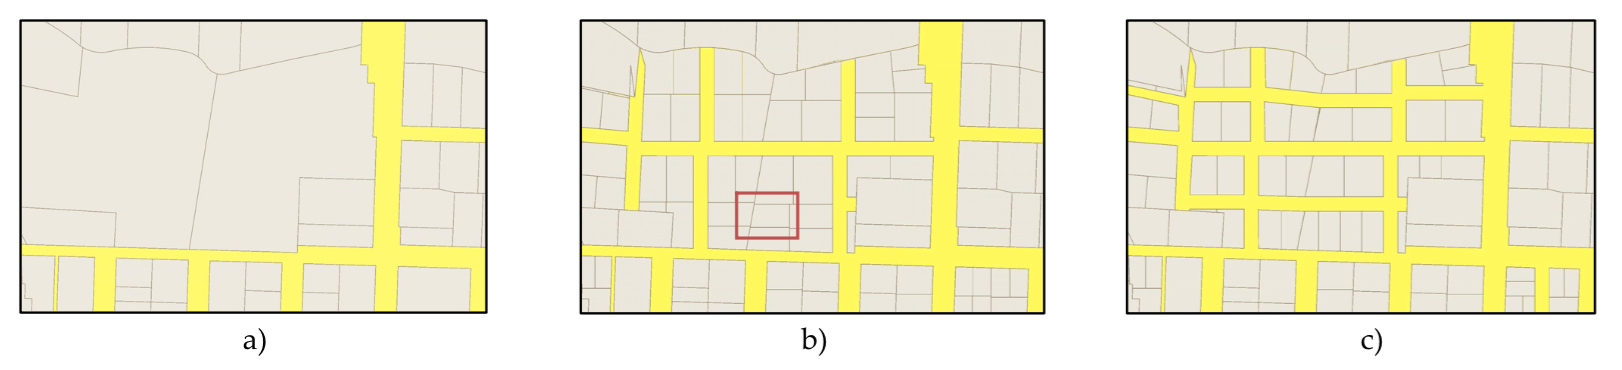
\includegraphics[width=0.9\linewidth]{star-5-5}
  \caption{\label{fig:star-5-5} \textbf{Geometry generation.} (a) Original area. (b) Automatic subdivision of the area. (c) Additional streets are generated in order to enforce egress rule.}
\end{figure*}

\begin{figure*}[htb]
  \centering
  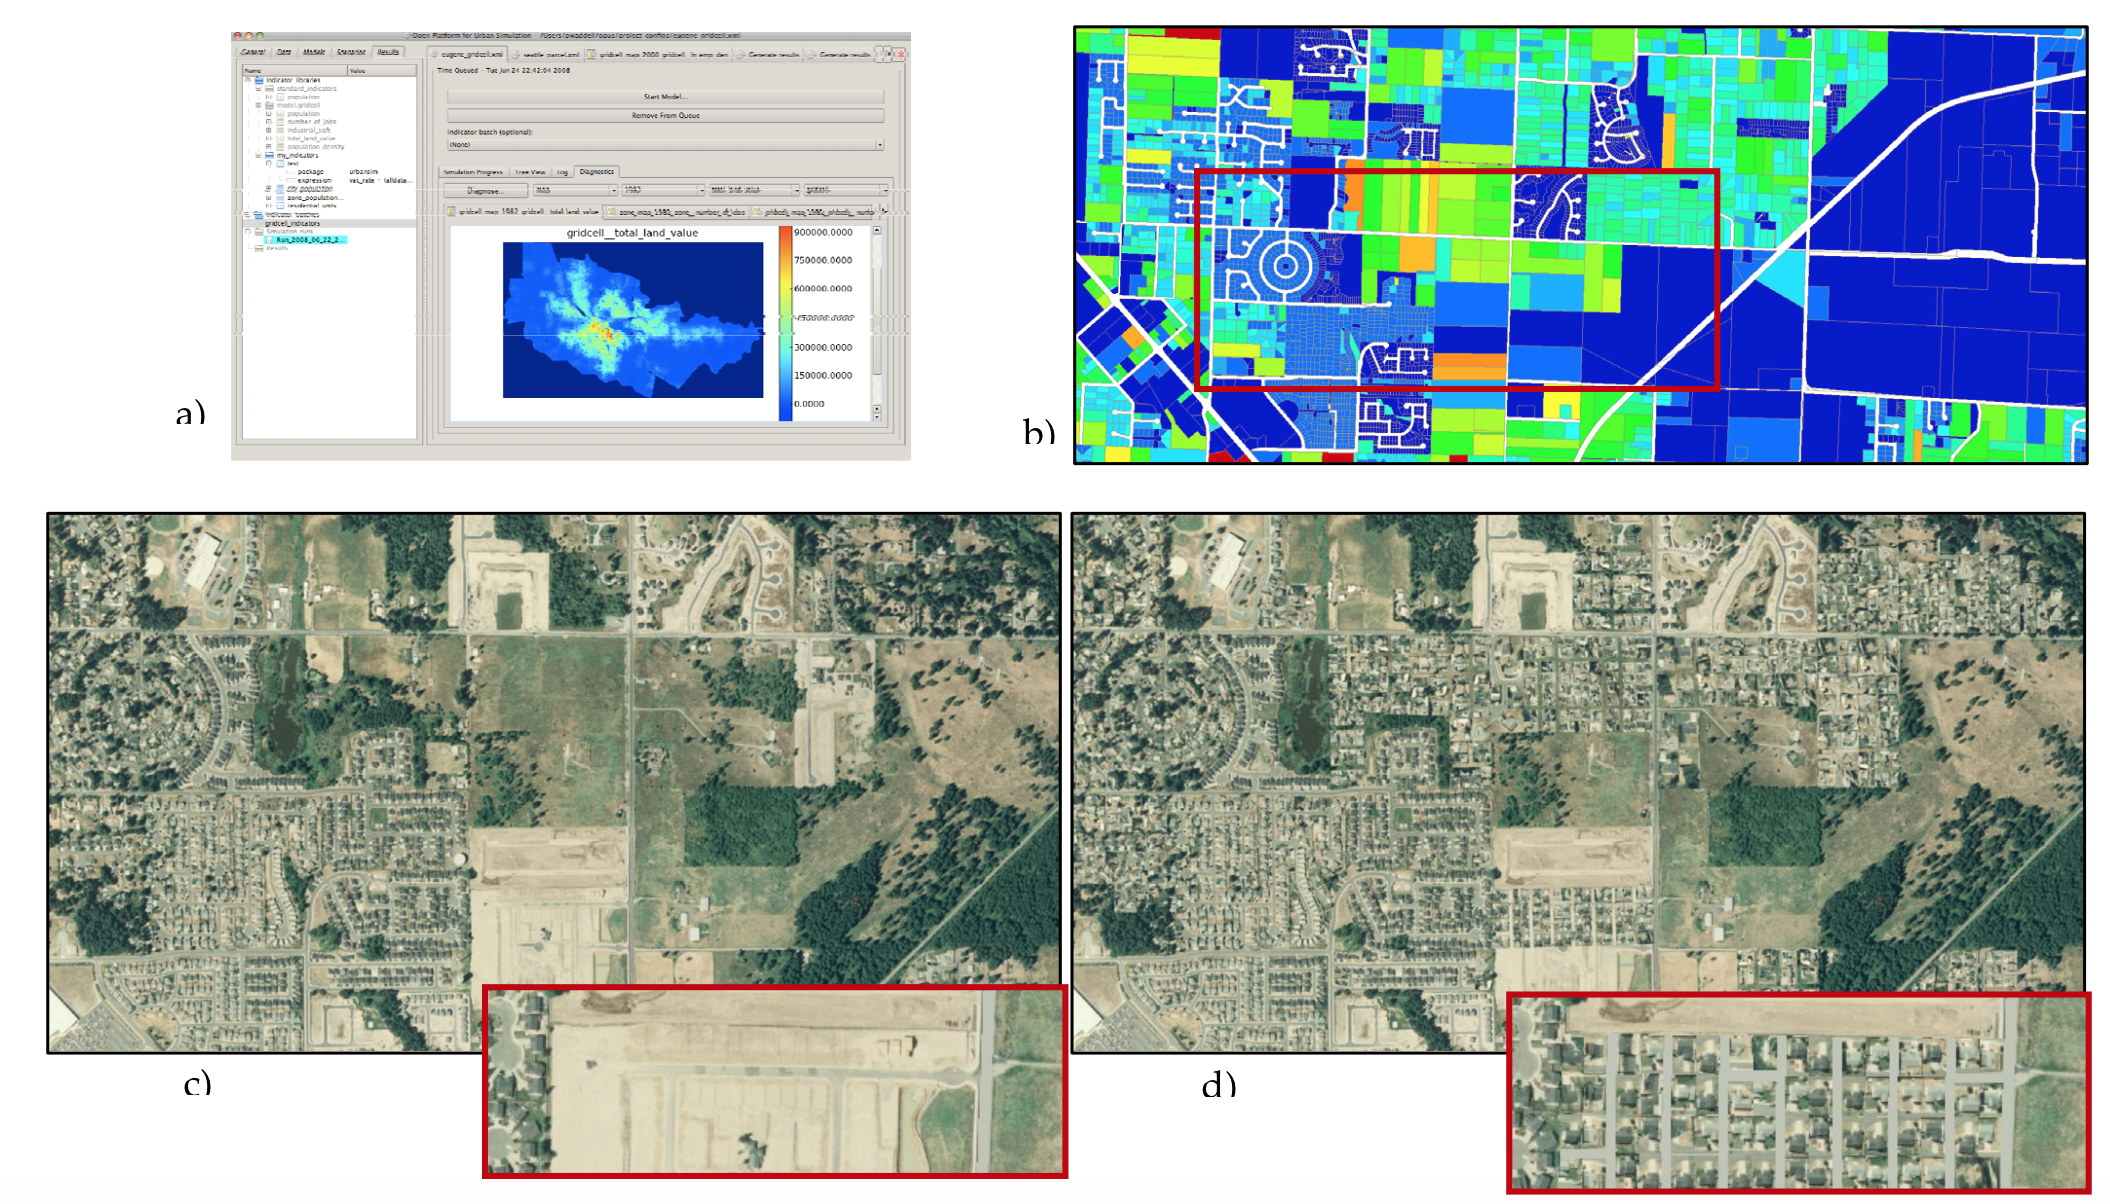
\includegraphics[width=.95\linewidth]{star-5-6}
  \caption{\label{fig:star-5-6} \textbf{Exemplary choroplethic visualizations of urban simulation data and views.} (a) A screen snapshot from the Indicator system supported by UrbanSim. (b) A rainbow color map used to represent changes in households/buildings for the initial set of parcels; blue corresponds to no change and green/yellow/red corresponds to a small/medium/large increase in the number of households. (c) The original layout of an urban area before the simulation and (d) generated layout after the simulation.}
\end{figure*}

\subsection{side note about urban simulation}

For more information about urban simulation modeling, please refer to the excellent overview by Waddell ~\cite{waddell2004introduction}.

The urban simulation tool used by ~\cite{vanegas2009visualization} is UrbanSim, a widely used software-based simulation system for supporting planning and analysis of urban development, incorporating the interactions between land use, transportation, the economy, and the environment. Overviews about UrbanSim can be found at ~\cite{waddell2002urbansim} and ~\cite{waddell2011integrated}.

There are multiple research projects ongoing that utilizes or extends UrbanSim, here we list some of such projects that are of particular importance:
\begin{itemize}
  \item \textbf{SustainCity Project} (http://www.sustaincity.org). This project is funded by the European Research Council and is seeking to develop an European-adapted version of UrbanSim (called UrbanSim-E) to make it more suitable for the context of European cities. The system was then tested in three European case studies: Brussels, Paris and Zurich.
  \item \textbf{FHWA: Modeling the Urban Continuum} (http://urbanmodel.asu.edu/intmod.html). This project is funded by the Federal Highway Administration, and focuses on 'Modeling the Urban Continuum in an Integrated Framework: Location Choice, Activity-Travel Behavior, and Dynamic Traffic Patterns'.
  \item \textbf{NSF: Robust Intelligence Project}. This project focuses on melding artificial intelligence techniques with discrete choice econometric methods to develop dynamic models of activity and routing behaviors.UC ITS Multi-Campus Research Program on Sustainable Transportation.
\end{itemize}

These projects, among some others, are part of a initiative that is intended to develop common data structures for urban modeling and 3D visualization.

%------------------------------------------------------------------------
\section{Interviews}

We interviewed two domain scientists to get first-hand information about their everyday research work and how visualization helps.

\subsection{Interview 1}

Interviewee: Dr. Nebiyou Tilahun, Assistant Professor, Department of Urban Planning and Policy, University of Illinois at Chicago

\textbf{What are the main research project(s) you work on?}

I work on questions of travel behavior, access, and the economic outcomes for people that are linked with the provision of transportation.

\textbf{What would be an ideal result from the project(s)?}

The ideal would be to be able to influence transportation policy that is consistent with travel behavior and decisions that allow for equitable access to opportunities.

\textbf{What kind of data do you work with most often in your research?}

I work with Census data, travel behavior data (such as Travel Tracker collected by CMAP, or Travel Behavior Inventory collected by Metro Council (Minnesota)), LEHD, Census CTPP. I have also collected data through surveys when needed.

\textbf{How do you gather or generate this data?}

Most are available through online portals by the collecting agency.

\textbf{How is this data used/analyzed?}

The data is used to do empirical work. Questions of choice are analyzed as a function of cost, service availability, land use, and other variables.

\textbf{What visualization tools/techniques do you use to help make sense of this data?}

Mostly statistical software to do plots and graphs. Another example is what we did for the accessibility project.

\textbf{What visualization tools/techniques do you use to display the data and/or communicate with other experts in your field?}

Mostly figures and plots done in R. On occasion made in Excel. They are presented using Powerpoint or Keynote.

\subsection{Interview 2}

Interviewee: Dr. Ning Ai, Assistant Professor, Department of Urban Planning and Policy, University of Illinois at Chicago

\textbf{What are the main research project(s) you work on?}

In general, my research focuses on \textbf{urban environmental planning}. I have three ongoing projects: (1) modeling the sustainability, resilience, and stability of urban systems in a metabolism framework (e.g., categorizing inputs and outputs of urban systems); (2) modeling food waste generation volume and recovery/reuse opportunities in urban neighborhoods; (3) investigating how healthcare sector can reduce greenhouse emissions through sustainable transportation programs.

\textbf{What would be an ideal result from the project(s)?}

Ideal outcomes would be deliverables that can benefit researchers, practitioners, and general public. That means the results should be publishable, transferable and replicable in other studies and regions, and accessible to the public.

\textbf{What kind of data do you work with most often in your research?}

Most often we use data on demography, land use, economy, ecology, and environment at various geographic and temporal scales.

\textbf{How do you gather or generate this data?}

We collect data from various government agencies, industry/market reports, as well as research publications, through online data/ literature reviews, formal surveys, and personal communications.

\textbf{How is this data used/analyzed?}

Data may be aggregated or disaggregated using spatial and statistical analyses. Advanced models may also need to be developed for environmental and socioeconomic impact analyses.

\textbf{What visualization tools/techniques do you use to help make sense of this data?}

ArcGIS Spatial Analyst/Network Analysis, MS Excel and Access.

\textbf{What visualization tools/techniques do you use to display the data and/or communicate with other experts in your field?}

ArcGIS, Photoshop, Adobe suites.

%-------------------------------------------------------------------------
\section{Conclusion}
There are many other fields in urban planning, including urban transportation, urban accessibility, urban modeling and so on. Much exciting work has been done in these directions. Due to the limit in space, we have to omit them. We hope in the future, we can conduct a more comprehensive survey of the state-of-the-art of more fields in urban planning.

%-------------------------------------------------------------------------

%\bibliographystyle{eg-alpha}
\bibliographystyle{eg-alpha-doi}

\bibliography{egbibsample}

%-------------------------------------------------------------------------

\end{document}